\documentclass[a4paper]{article}

\usepackage{fullpage} % Package to use full page
\usepackage{parskip} % Package to tweak paragraph skipping
\usepackage{tikz} % Package for drawing
\usepackage{amsmath}
\usepackage{hyperref}
\usepackage{pythonhighlight}

\title{TD - Information Extraction from Wikipedia pages}
\author{Adrianna Janik}


\begin{document}

\maketitle

\section{Introduction}
Knowing that most of the world including Web data are unstructured for example: text, speech or images, there is a need for having a way for retrieving structured information from this kind of data. Following Wikipedia we know that \textit{Information extraction (IE) is the task of automatically extracting structured information from unstructured and/or semi-structured machine-readable documents.} Among possible applications of IE we can find Question Answering / Structured Queries
for example: \textit{Which companies are releasing new smartphones new products in Europe this Spring?} or \textit{Alert me anytime a new smartphone is announced in the U.S.}. In Data Mining we can analyze trends in product releases across different industries or answer questions like \textit{Is there a correlation between price and date of release?}. We can distinguish 3 main methods of IE: 
\begin{enumerate}
\item Hand-written regular expressions
\item Using classifiers
\item Sequence models
\end{enumerate}
\cite{slides}

\section{Goal of the TD}
In this TD we were annotating and retrieving information from Wikipedia articles. Given as arguments:
\begin{itemize}
	\item a set of Wikipedia articles, and
	\item a file with a list of entities and their uri 
\end{itemize}

We had to implement an algorithm that annotates the mentions of entities in the content of articles. Then we had to extract information about birth day of entity if applicable and normalize the extracted dates to the form YYYY-MM-DD. Next step was to extract information about the type of the article entity and finally find a pattern in Wikipedia, given a seed fact like 'is married to'. Because of limited amount of data and introductory character of this TD we were using hand-written regular expressions to extract informations from articles.

\section{Tools}
To extract information from articles and annotate them with proper links I used Python along with some libraries like regular expression library, urllib, gender\_guesser, nltk, os... \\
To run the script we should first install proper packages for Python 3.5.2:
\begin{itemize}
\item attrs==17.4.0
\item clize==4.0.3
\item docutils==0.14
\item gender-guesser==0.4.0
\item lxml==4.1.1
\item nltk==3.2.5
\item numpy==1.14.1
\item od==1.0
\item pyparsing==2.2.0
\item python-dateutil==2.6.1
\item python-gantt==0.6.0
\item sigtools==2.0.1
\item six==1.11.0
\item svgwrite==1.1.12
\end{itemize}	


\section{Algorithm}
Our program consists of main class Annotator and several helper functions and data structures. \\

At the top of extraction script we should put necessary imports and data structures declarations: \\
\begin{python}
from urllib import parse
import os
import nltk
import re
import gender_guesser.detector as gender
from datetime import date
import datetime
import calendar as cal 


dg = {"female": "she her", "male": "he his", "unknown":"he she his her", "mostly_male": "he his", "mostly_female": "she her", "andy": "he she his her"}
gg = {"female": "she", "male": "he", "unknown":"", "mostly_male": "he", "mostly_female": "she", "andy": "he she"}

genders = {}
genders_person = {}
    \end{python}


First step is to extract dictionary of entities from the file, this can be done with the usage of below function: \\

\begin{python}
def get_dict_of_entities():
    entities = {}
    g = gender.Detector()

    with open('./TD/entity_list.txt') as f:
        for line in f:
           tmp = parse.urlparse(line).path.split('/')[-1].strip().replace('_',' ')
           try:
               ind = tmp.index("(")
               tmp = tmp[:ind]
           except:
               pass
           entities[tmp] = line.strip()
           genders[tmp] = dg[g.get_gender(tmp.split()[0])]
           genders_person[tmp] = gg[g.get_gender(tmp.split()[0])]
   
    return entities
\end{python}

Next we have to define main class of the script called Annotator, this class will contain all the logic necessary to extract and annotate data from Wikipedia.

\begin{python}
class Annotator:
    def __init__(self, path='./TD/Wikipedia_corpus'):
        self.path = path
        self.entities = get_dict_of_entities()
        self.knowledge = []

\end{python}

Methods of Annotator class:
\begin{itemize}
\item get\_list\_of\_files()
\item annotate()
\item annotate\_files()
\item extract\_birth\_day()
\item extract\_type()
\item extract\_pattern()
\item extract\_marriage()
\end{itemize}

In below function we retrieve all file names from Wikipedia corpus.
\begin{python}
    def get_list_of_files(self):
        return os.listdir(self.path)
\end{python}

The core function of Annotator class as well as the whole script is function annotate it is used to annotate and extract data from a single file. It accepts as an argument file name and process it. Annotated file is then saved in special folder called Annotations and its name is name\_of\_original\_file\_ant.txt. This function calles several other functions called extractors for different parts of data that need to be retrieved but those functions will be described later. Here we mainly annotate data with a simple regex function \cite{regex}  that firstly looks for the full name of entity and then for only the surname and pronouns that are applicable to this entity. To get matching pronouns I used package gender\_guesser that allows to get gender based on the person name to access pronouns I created a dictionary gg in which for each gender proper pronouns are set. At the end detected patterns in text are substituted with proper entity annotations.
\begin{python}
    def annotate(self, file_name):
        with open('./TD/Annotations/' + file_name.replace('.txt','_ant.txt'), 'w') as fw:
            with open(self.path + '/' + file_name) as fr:
                text = fr.read()
                for item in self.entities:
                    if check_if_valid(text, item):
                        self.knowledge.append(self.extract_birth_day(text, item))
                        self.knowledge.append(self.extract_type(text, item))
                        self.knowledge.append(self.extract_pattern(text, item))
                        self.knowledge.append(self.extract_marriage(text, item))
                        self.knowledge.append(self.extract_pattern(text, item, pattern="appeared in"))

                        tmp = item.split(' ')
                        name = tmp[0].strip()
                        g = gender.Detector()
                        pronouns = genders_person[item].split()
                        pros = pronouns + [x.title() for x in pronouns]
                        regex = "(" + item + "|" + tmp[-1].strip() + "| " + " |".join(pros)  + " )"
                        text = re.sub(regex, r'<entity name="'+self.entities[item]+'">\\1</entity>', text)
            fw.write(text)

\end{python}

Function that collects extracted data and calles above function for every file is presented below and its called annotate\_files(). Collected data are stored in class property knowledge and here it is saved to the file called 'knowledge.xml' in a XML format.
\begin{python}
    def annotate_files(self):
        files = self.get_list_of_files()
        for f in files:
            self.annotate(f)
        with open("knowledge.xml","w") as f:
            f.write('<?xml version="1.0" encoding="UTF-8"?>\n<data>')
            f.write('\n'.join(list(filter(lambda x: x != "", self.knowledge))))
            f.write("</data>")

\end{python}

At last there are functions that are used specially to extract specific data from articles. Next function is used for extracting birth dates from people from articles. It is based on regex that searches for patterns starting from two words with capital letters representing name and surname, then in some cases there are some other informations about the person that we want to ignore and limit it only to 60 characters. Next we can have two form of birth dates with keyword 'born' and only with dates of birth and death in brackets. After data is extracted with regex function findall - date is converted to format: YYYY-MM-DD and proper knowledge entity is created with data about birth date. This is returned to the annotate() function.
\begin{python}
    def extract_birth_day(self, text, entity):

        regex = r"(?P<person>(?:[A-Z][a-z]+\s){2})(?:.){0,60}?(?:\(?born )?(?:\(?born (?P<year>\d\d\d\d)\)?|(?:(?P<day_base>\d\d?) (?P<month_base>[A-Z][a-z]*) (?P<year_base>\d\d\d\d)\)?))"
        extract = ""
        tmp = re.findall(regex, text)
        if tmp:
            year = 1000
            month = 1
            day = 1
            if tmp[0][1] != "":
                year = int(tmp[0][1])
                dat = date(year, month, day).strftime("%Y")

            else:
                year = int(tmp[0][4])
                day = int(tmp[0][2])
                month = list(cal.month_name).index(tmp[0][3])
                dat = date(year, month, day).strftime("%Y-%m-%d")

            print(dat)
            extract = '<entity link="' + self.entities[entity] + '" hasDate= "' + dat + '"/>'
        return extract

\end{python}

Function for extracting type of the entity is similar to the previous one, it is also based on regex but also after regex there is extra validation performed to check if what was detected is a noun with possible description in the form of adjectives/ or verb in gerund separated with conjunctions or commas. As previously proper entity is created and returned to annotate() function.
\begin{python}
    def extract_type(self, text, entity):
        det = ""
        regex = r"(.*?)(?:is|are|was|were) (?:a|the|an) (.*)"
        tmp = re.findall(regex, text)
        for i in tmp:
            if check_if_valid(i[0], entity):
                words = nltk.word_tokenize(i[1])
                tokens = nltk.pos_tag(words)
                detected_type = entity.title()
                for tok in tokens:
                    if "NN" in tok[1]:
                        det += " " + tok[0]
                    elif "JJ" in tok[1]:
                        det += " " + tok[0]
                    elif "VBG" in tok[1]:
                        det += " " + tok[0]
                    elif "," in tok[1]:
                        det += ""
                    elif "CC" in tok[1]:
                         det += ""
                    else:
                        break
                detected_type += " is " + det
                print(detected_type)
            break
        extract = '<entity link="' + self.entities[entity] + '" type="' + det + '"/>'
        return extract

\end{python}

Last two functions are almost the same with one difference that extract\_pattern is more general and extract\_marriage is only used to extract information about marriage in several form with more details. It is also based on regex and it allows to detect the 'subject' of marriage described with other words of proper types. As in previous function extracted data is returned to annotate() function.

\begin{python}
    def extract_pattern(self, text, entity, pattern="painted"):
        det = ""
        extract = ""
        regex = r"(.*?)(?:" + pattern + ") (.*)"
        tmp = re.findall(regex, text)
        for i in tmp:
            if check_if_available(i[0], entity):
                words = nltk.word_tokenize(i[1])
                tokens = nltk.pos_tag(words)
                detected_type = entity.title()
                for tok in tokens:
                    if "NN" in tok[1]:
                        det += " " + tok[0]
                    elif "JJ" in tok[1]:
                        det += " " + tok[0]
                    elif "VBG" in tok[1]:
                        det += " " + tok[0]
                    elif "," in tok[1]:
                        det += ""
                    elif "CC" in tok[1]:
                         det += ""
                    elif "DT" in tok[1]:
                         det += ""
                    else:
                        break
                if det != "":
                    detected_type += " " + pattern + " " + det
                    print(detected_type)
                    if det in self.entities:
                        extract = '<entity link="' + self.entities[entity] + '" ' + "_".join(pattern.lower().split()) + '= "' + self.entities[det] + '"/>'
                    else:
                        extract = '<entity link="' + self.entities[entity] + '" ' + "_".join(pattern.lower().split()) + '="' + det + '"/>'

        return extract

\end{python}

\begin{python}
    def extract_marriage(self, text, entity):
        det = ""
        extract = ""
        regex = r"(.*?)(?: is|are|was|were|(?:has been))? (?:married|marriage to) (.*)"
        tmp = re.findall(regex, text)
        for i in tmp:
            if check_if_available(i[0], entity):
                words = nltk.word_tokenize(i[1])
                tokens = nltk.pos_tag(words)
                detected_type = entity.title()

                for tok in tokens:
                    if "NN" in tok[1]:
                        det += " " + tok[0]
                    elif "JJ" in tok[1]:
                        det += " " + tok[0]
                    elif "VBG" in tok[1]:
                        det += " " + tok[0]
                    elif "," in tok[1]:
                        det += ""
                    elif "CC" in tok[1]:
                         det += ""
                    else:
                        break
                if det != "":
                    detected_type += " is/was married to " + det
                    print(detected_type)
                    if det in self.entities:
                        extract = '<entity link="' + self.entities[entity] + '" ' + "married_to" + '="' + self.entities[det] + '"/>'
                    else:
                        extract = '<entity link="' + self.entities[entity] + '" ' + "married_to" + '="' + det + '"/>'

            break

        return extract

\end{python}

%\begin{python}
%\end{python}


\section{Results}
For extracted dates now for example we can draw a timeline of birth days for each person in the dataset. It is much easier then extracting dates manually from the articles.

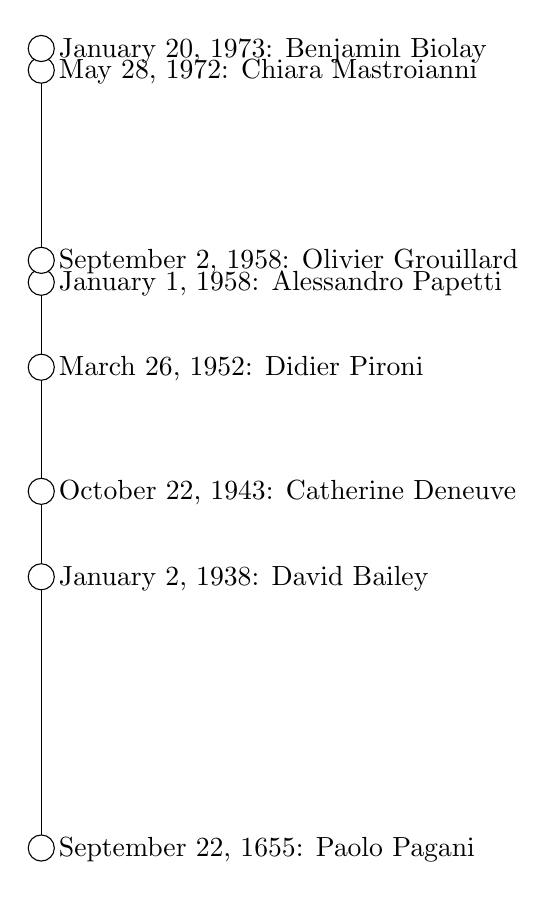
\begin{tikzpicture}[datemarker/.style={circle,draw=black,fill=white,radius=4pt},
textlabel/.style={anchor=west,text height=1.7ex,text depth=.25ex}]
\draw (0,0) -- (0,10);
\node at (0, 0.0) [datemarker] {};
\draw (0.1, 0.0) node [textlabel] {September 22, 1655: Paolo Pagani};
\node at (0, 3.444683930013062) [datemarker] {};
\draw (0.1, 3.444683930013062) node [textlabel] {January 2, 1938: David Bailey};
\node at (0, 4.529726482137911) [datemarker] {};
\draw (0.1, 4.529726482137911) node [textlabel] {October 22, 1943: Catherine Deneuve};
\node at (0, 6.105828877343332) [datemarker] {};
\draw (0.1, 6.105828877343332) node [textlabel] {March 26, 1952: Didier Pironi};
\node at (0, 7.18472678075393) [datemarker] {};
\draw (0.1, 7.18472678075393) node [textlabel] {January 1, 1958: Alessandro Papetti};
\node at (0, 7.463284189133316) [datemarker] {};
\draw (0.1, 7.463284189133316) node [textlabel] {September 2, 1958: Olivier Grouillard};
\node at (0, 9.87864318789354) [datemarker] {};
\draw (0.1, 9.87864318789354) node [textlabel] {May 28, 1972: Chiara Mastroianni};
\node at (0, 10.153616217856278) [datemarker] {};
\draw (0.1, 10.153616217856278) node [textlabel] {January 20, 1973: Benjamin Biolay};
\end{tikzpicture} \\

For this purpose I created a custom version of timeline drawing script presented here \cite{timeline}. Which allows to visualize dates in a form of timeline.

\section{Conclusions}

In this report I have explained an algorithm for extracting informations from Wikipedia articles and annotating it with proper entities.
We could see that information extraction is useful for analysing and visualising data that is unstructured for example with a simple timeline.
There are various other aspects that could be explored here for example running the script for bigger number of articles or creating bigger list of patterns to be detected.

\bibliographystyle{plain}
\bibliography{bibliography}
\end{document}
